% Standardinkluderingsfil
%
%  untitled
%
%  Created by David Granqvist on 2008-09-08.
%  Modified by Martin Erola
%

% Set document format/class
\documentclass[a4paper,twoside]{article}

%%%%%%%%%%%%%%%%%%%
% Include packages
%
\usepackage[utf8]{inputenc}   % Use utf-8 encoding for foreign characters
\usepackage[swedish]{babel}   % Support for swedish letters
\usepackage{fullpage}         % Setup for fullpage use
\usepackage{fancyhdr}         % Running Headers and footers
\usepackage{boxedminipage}    % Surround parts of graphics with box
\usepackage{listings}         % Package for including code in the document
\usepackage{ifpdf}            % Recommended way for checking for PDFLaTeX:
\usepackage{tabularx}         % Tabeller med automatisk stretch
% \usepackage[nofancy]{svninfo} % Extract Subversion info about the file
% \usepackage{color}          % Color
% \usepackage{lastpage}       % Total page count

% Graphics
\ifpdf
\usepackage[pdftex]{graphicx}
\else
\usepackage{graphicx}
\fi

%%%%%%%%%%%%%%%%%%%%%%%%%%%%%%%%%%%%%%%%%%%%%%%%%%%%%%%%%%
% Uncomment some of the following if you use the features
%

% Multipart figures
%\usepackage{subfigure}

% More symbols
%\usepackage{amsmath}
%\usepackage{amssymb}
%\usepackage{latexsym}

% If you want to generate a toc for each chapter (use with book)
% \usepackage{minitoc}

%%%%%%%%%%%%%%%%%%%%
% Document settings
%

% Header
\pagestyle{fancy}
% Sätter en marginal mellan header och (ovanstående?) text %
\setlength\headsep{10pt}
% Sätter höjden på headern
\setlength{\headheight}{32pt}

% Sätter styckesinställningar
\setlength\parindent{0pt}
\setlength\parskip{10pt}



\ifpdf
  \DeclareGraphicsExtensions{.pdf, .jpg, .tif, .png}
  \pdfinfo{            
    /Title  (Architecture Notebook)
    /Author (PUM-grupp 1)
  }
\else
  \DeclareGraphicsExtensions{.eps, .jpg}
\fi

\title{Distribuerad wiki \\ Architecture Notebook}
\author{PUM-grupp 1}
\date{\today}

\begin{document}

\maketitle

\thispagestyle{empty}

\newpage

{\centering \Large{Dokumenthistorik\\}}

\vspace{10pt}
\begin{tabularx}{\textwidth}{ |l|l|X|l|l| }
  \hline
    \textbf{version} & \textbf{datum} & \textbf{utförda ändringar} & \textbf{utförda av} & \textbf{granskad} \\
	\hline 
  0.1 & 2009-02-12 &  Ett första utkast  & Alla & Alla   \\
	\hline 
  0.2 & 2009-02-12 &  Arkitekturen utvecklad ytterligare  & Alla & Alla   \\
  \hline
\end{tabularx}

\newpage

\setcounter{tocdepth}{2}
\tableofcontents
\newpage

\section{Syfte}
Detta dokument syftar till att beskriva de filosofier och motiveringar som står till grund för det arkitekturella ramverket för projektet.
\section{Arkitekturella mål och filosofi}
Arkitekturen i projektet styrs främst av de krav som har stipulerats.
\section{Antaganden och beroenden}
I denna sektion nämns de antaganden och beroenden som finns och som tillsammans bygger upp en bild över hur programvaran kommer byggas.
\begin{itemize}
\item Systemet ska fungera på Linux
\item Systemet ska fungera decentraliserat
\item Systemet ska kunna kommunicera via nätverk
\item Systemet ska lagra data lokalt
\end{itemize}
\section{Arkitekturellt signifikanta krav}
Här kommer referenser till krav i andra dokument att finnas.
\section{Beslut, begränsningar och motiveringar}
Här är en lista med beslut, begränsningar och tillhörande motiveringar.
\begin{itemize}
\item Bazaar används som distributionssystem, eftersom det är lätt att integrera.
\end{itemize}
\section{Arkitekturen}
I den här sektionen beskrivs arkitekturen övergripande, med mer
detaljerade beskrivningar i respektive moduls sektion.

\begin{figure}[ht]
  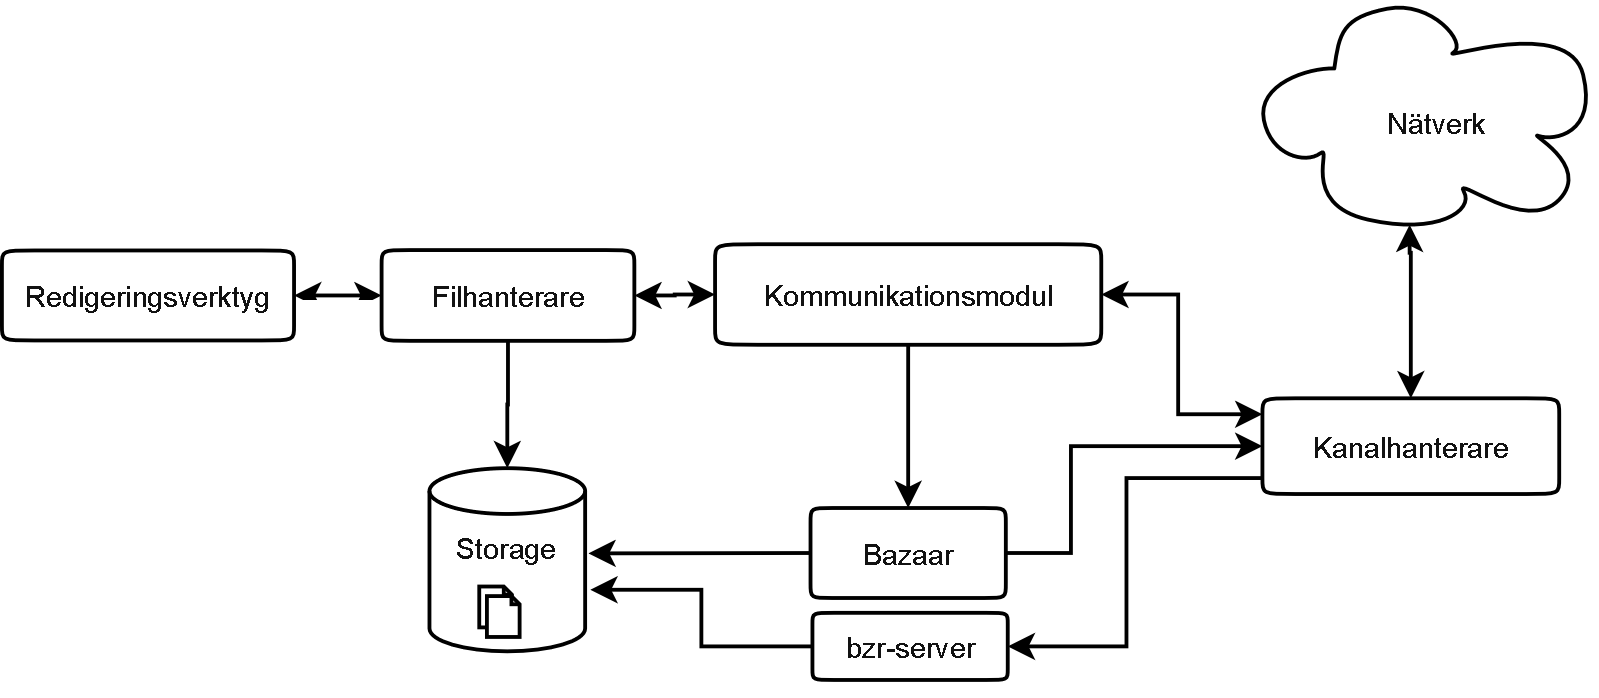
\includegraphics[width=160mm]{Architecture-diagram.png}
  \caption{Diagram över arkitekturen}
  \label{fig1}
\end{figure}

Kommunikationsmodulen är central i systemet, och tillhandahåller
kommunikationsmöjligheter mellan klienten,
distribueringsundersystemet, redigeringsverktyget och andra klienter.

För kommunikation klienter emellan används TLS över TCP/IP. En av
klienterna ansluter till den andra och TLS-handskakning och
autenticering genomförs.

Det underliggande distributionssystemet som vi använder är Bazaar. För
att kunna slå ihop två personers repositorier kommunicerar den ena
klientens Bazaar-klient med den andras Bazaar-server över
TLS-anslutningen via kommunikationsmodulen.

En filhanterare agerar som lager mellan redigeringsverktyget och
kommunikationsmodulen. Denna tillhandahåller en modell för att hålla
filhanteraren och kommunikationsmodulen underrättade om händelser i
andra delar av systemet. Filhanteraren arbetar också mot arbetsmappen
och tillhandahåller metoder för att modifiera filer mot
denna. Kommunikationsmodulen via distributionssystemet tillhandahåller
metoder för att distribuera modifieringar som sker i arbetsmappen.
\section{Arkitekturella mekanismer}
I denna sektion nämns de olika mekanismerna som driver
programvaran. Dessa kommer få mer detaljerade beskrivningar under
senare iterationer.
%\subsection{Säkerhet}
%Som en del av programvarans specifikation nämns säkerhet mellan
%klienterna. Informationens integritet ska vidbehållas, alltså skyddas
%mot olovlig ändring vid informationsöverföringar samt vid lagring på
%hårddisk.
%\begin{itemize}
%\item Mellan vilka arkitekturella moduler och i vilka instanser är säker kommunikation nödvändig?
%\item Vilken data är relevant att kryptera eller verifiera?
%\item Hur stort fokus ska läggas på datasäkerhet?
%\item Strider åtgärderna för ökad sökerhet mot andra krav såsom tillgänglighet?
%\end{itemize}
\subsection{Felsökning}
Programvaran kommer med största sannolikhet behöva felsökas under
utvecklingstiden. Felsökning kommer vara relevant i många delar av
programvaran.

Felsökning kan ske passivt och aktivt. Aktivt genom att till exempel
stega kod under körning. Passivt genom loggning.

Frågor rörande felsökning som kommer utvecklas senare i projektet följer nedan.
\begin{itemize}
\item I vilka instanser kommer felsökning att vara relevant?
\item Vilka felsökningsmetoder och verktyg skall användas?
\item Hur stora datamängder behöver loggas?
\item Hur ska loggning ske utan att användarens integritet kränks?
\end{itemize}
\subsection{Lagring}
Lagringsmekanismen är den mekanism som sköter den lokalt lagrade datan
hos alla klienter.

För närvarande utgörs lagringsmodulen av Bazaar och det underliggande
filsystemet som Python tillhandahåller. Bazaar tillhandahåller en
historik om filer i systemet. De inbyggda distributionsmekanismerna i
Bazaar används, varför ingen särskild mekanism för läs- och
skrivrättigheter för lagringsmekanismen krävs.

Ytterligare frågor rörande lagringsmekanismen är som följer.
\begin{itemize}
\item Hur mycket utrymme krävs på den lokala hårddisken?
\item Vad händer om hårddiskutrymmer tar slut?
\item Vad händer om en delmängd av allt data tas bort eller blir korrupt?
\end{itemize}
\subsection{Distribution}
Distributionsmekanismen är den som sköter synkroniseringen klienterna
emellan. Den ser till att uppdateringar sprider sig över nätverket
till alla andra klienter som arbetar online.

Som distrubitionsmodul är Bazaar vald. Denna går lätt att integrera
med Python då den är skriven i densamma samt tillhandahåller ett
heltäckande och väldokumenterat gränssnitt för initiering,
manipulering och distribution av repositorier.

Bazaar tillhandahåller en historia över ändringar som skett och har
möjlighet att återskapa ett dokument när som helst i tid. När
konflikter uppstår flaggas den berörda filen. Distributionsmodulen ser
då till att de orsakande parterna informeras om konflikten så att de
kan lösa den. Om en av parterna är den lokala användaren informeras
denna via användargränssnittet, annars publiceras konflikten i det
lokala nätverket.

Relevanta frågor som rör distribuering följer.
\begin{itemize}
\item Hur ofta skall synkronisering ske?
\item Vad händer om en användare bryter en pågående distribution?
\end{itemize}
\subsection{Kommunikation}
Kommunikationsmodulens uppgift består i att upprätta kommunikation
mellan klienter och att arbeta som ett mellanled mot
distributionstekniken.

För säker kommunikation används TLS. Denna anslutningsmetod klarar av
att kryptera datatrafik och autentisera användare.

För att möjliggöra distribution över TLS-anslutningen tillhandahåller
kommunikationsmodulen emulerade portar, som från den lokala datorn går
via TLS-anslutningen till mottagarklienten. Detta innebär att
distribueringen kan ske dubbelriktat även om den ena av klienterna
ligger bakom en brandvägg.

\begin{itemize}
\item Vilka krav skall ställas på kommunikationskanalens karaktäristika?
\end{itemize}
\subsection{Redigering}
Redigeringsmodulen finns lokalt hos klienten och tillåter användaren
att redigera wiki-sidor via ett grafiskt gränssnitt.

När användaren redigerat klart sparas ändringen till det lokala
versionshanteringssystemet och distributionsmodulen informeras om
uppdateringen.
\subsection{Bläddring}
Bläddringsmodulen går ut på att visa wiki-sidor för
användaren. Användaren kan använda bläddringsmodulen för att utforska
sin lokala kopia av den distribuerade wikin. När ändringar sker i
sidor som är i vy ser bläddringsmodulen till att uppdateringarna
presenteras till användaren på ett enkelt och tydligt sätt.
\section{Huvudabstraktioner}
Här definieras de abstraktioner som används för att beskriva systemet.
\subsection*{Användare}
En användare är en person i systemet. 
\subsection*{Klient}
En klient är en instans av programvaran som körs aktivt på någon
plattform. En användare kan inneha en klient.
\subsection*{Nyckel}
En datamängd som används för signering, verifiering och säker kommunikation.
\section{Arkitekturellt ramverk}
Det arkitekturella ramverket definierar hur systemet är
sammansatt. Ramverket definieras bättre under senare delar av
projektet.
\end{document}
